\documentclass[12pt]{article}
\usepackage[svgnames,x11names,table]{xcolor}
\usepackage{hyperref}
\usepackage{graphicx}
\usepackage{parskip}
\usepackage{float}
\usepackage{amsmath}
\usepackage{amssymb}
\usepackage{enumitem}
\usepackage[thicklines]{cancel}

\hypersetup{
    colorlinks,
    citecolor=blue,
    filecolor=black,
    linkcolor=black,
    urlcolor=RoyalBlue4,
}

\title{Creating a Simple Vector Calculus Framework to Verify Stokes' Curl Theorem}
\author{Mohamed Hussien El-Deeb (201900052)}
\date{\today}

\begin{document}

\maketitle
\tableofcontents
\hypersetup{linkcolor=RoyalBlue4}

\newpage
\section{Introduction}

Stokes' curl theorem, also known as the Kelvin-Stokes theorem after \href{https://en.wikipedia.org/wiki/Lord_Kelvin}{Lord Kelvin} and
\href{https://en.wikipedia.org/wiki/Sir_George_Stokes,_1st_Baronet}{George Stokes}, is a theorem in vector calculus on \({\displaystyle \mathbb {R} ^{3}}\). Given
a vector field, the theorem relates the integral of the curl of the vector field over some
surface, to the line integral of the vector field around the boundary of the surface. This theorem can be
stated as: The line integral of a vector field over a loop is equal to the surface
integral of its curl over the enclosed surface. This unlocks integration shortcuts that greatly simplifies other theorems and speeds up computations.
This project is an attempt to build a simple vector calculus framework to verify and visualize
Stokes' curl theorem using basic numerical methods and the web graphics library \href{https://threejs.org/}{three.js}.

\newpage
\section{Stokes' Curl Theorem}
\subsection{Definition}

Stokes' theorem states that the line integral of a vector field \(\mathbf{F}\) around a closed curve \(C\) is equal to the surface integral of the curl of \(\mathbf{F}\) over any surface \(S\) bounded by \(C\). Mathematically, the theorem can be stated as:

\[
    \oint_{C} \mathbf{F} \cdot d\mathbf{r} = \iint_{S} (\nabla \times \mathbf{F}) \cdot d\mathbf{S}
\]

where:

\begin{itemize}
    \item \(\mathbf{F}\) is a differentiable vector field.
    \item \(C\) is a piecewise-smooth, positively oriented simple closed curve in space.
    \item \(S\) is a piecewise-smooth, positively oriented surface in space bounded by \(C\).
    \item \(d\mathbf{r}\) is the differential arc vector along \(C\).
    \item \(d\mathbf{S}\) is the differential area vector of \(S\).
\end{itemize}

\newpage
\section{Integration over a Path}

\subsection{Definition}

Since computers are discrete, we need to approximate the integral of a function over a path using numerical methods which means we will revert to using summation instead of integration while noting the values converge as the step size decreases.

Suppose we want to sum up the values of a function \(f(x, y, z)\) along a path \(C\) in space.

\[
    C = \left\{P(t) = \left\langle x(t), y(t), z(t)\right\rangle \mid 0 \leq t \leq 1\right\}
\]

We can approximate the path by dividing it into many small line segments and approximate the function by a constant value over each segment.
The sum of the values of the function over all segments is the integral of the function over the path.
Numerically, the integral can be approximated by the following formula:

\[
    \sum_{i=0}^{n} f(L_i)
\]

where:

\begin{itemize}
    \item \(f\) is the function to be integrated.
    \item \(L_i\) is a small line segment on the path.
    \item \(n\) is the integer number of line segments.
\end{itemize}

\(L_i\) is defined as follows:

\[
    L_i = \left[C\left(i \Delta t\right), C\left((i + 1)\Delta t\right)\right]
\]

where:

\begin{itemize}
    \item \(C(t)\) is the parametric equation of the path.
    \item \(\Delta t\) is the step size.
\end{itemize}

We can choose our parameter \(t\) to be \(0 \leq t \leq 1\) meaning we can substitute \(\Delta t\) with
\(\frac{1}{n}\).

Note that it is possible to convert parameter limits from \([a, b]\) to \([0, 1]\) using the following formula as long as \(a \neq b\):

\[
    P(t), \quad a \leq t \leq b \quad \rightarrow \quad P\left(\frac{t - a}{b - a}\right), \quad 0 \leq t \leq 1
\]

Now we arrive at the following formula:

\[
    \sum_{i=0}^{n} f\left(L_i\right)
\]

\[
    L_i = \left[C\left(\frac{i}{n}\right), C\left(\frac{i + 1}{n}\right)\right]
\]

The higher the value of \(n\), the more accurate the approximation.

\subsection{Implementation}

As a proof of concept, we can implement the path integral of a scalar field in three.js\cite{El-Deeb_PEU-218_Stokes_Threejs}. All example code is
part of the implementation software and can be found in the repository\cite{El-Deeb_PEU-218_Assignments}. Note that knowledge of three.js and computer graphics is required to understand the code.

\begin{figure}[H]
    \centering
    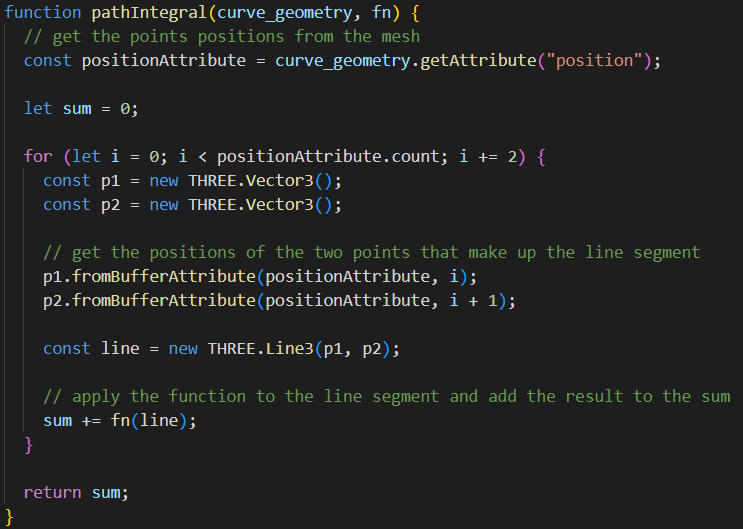
\includegraphics[width=0.8\textwidth]{images/path_int.png}
    \caption{Path Integral of a Scalar Field\cite{El-Deeb_PEU-218_Stokes_Threejs}}
\end{figure}

As it can be seen, the path integral of a scalar field is approximated by summing up the values of the scalar field over many small line segments on the path.
The boundary path itself is constructed using the edge geometry in three.js.

\begin{figure}[H]
    \centering
    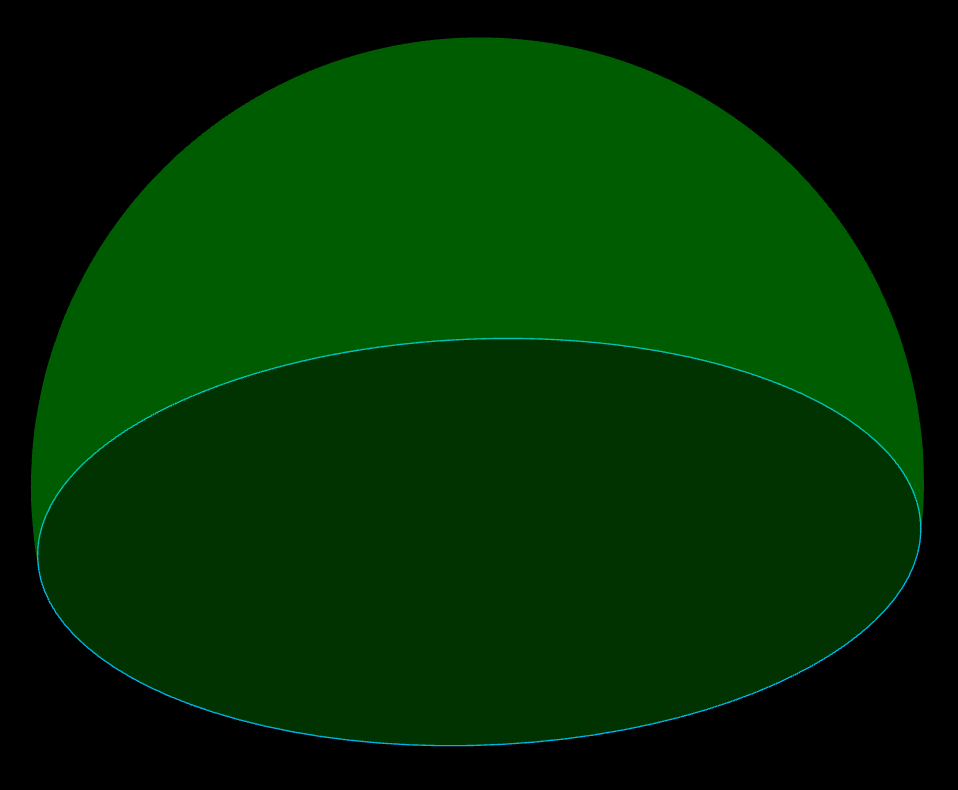
\includegraphics[width=0.8\textwidth]{images/path.png}
    \caption{boundary path of the surface of half a sphere\cite{El-Deeb_PEU-218_Stokes_Threejs}}
\end{figure}

This integration method is used to compute the path integral side of Stokes' curl theorem.

\newpage
\section{Integration over a Surface}

\subsection{Definition}

Similarly, we can approximate the integral of a function \(f(x, y, z)\) over a surface \(S\) using numerical methods.
We can divide the surface into small triangles and approximate the function by a constant value over each triangle.
The sum of the values of the function over all triangles converges to the integral of the function over the surface
as the limit of the step size reach 0.

To construct our triangle mesh, we can use the parametric equation of the surface \(S(u, v)\) where \(0 \leq u \leq 1\) and \(0 \leq v \leq 1\).
and sample the surface at \(n \times m\) points.

\[
    S(u, v) = \left[x(u, v), y(u, v), z(u, v)\right]
\]

\[
    T_{ij} = \left[S\left(i \Delta u, j \Delta v\right), S\left((i + 1)\Delta u, j \Delta v\right), S\left(i \Delta u, (j + 1) \Delta v\right)\right]
\]

For the sake of simplicity, we can assume \(\Delta u = \Delta v = \frac{1}{n}\).

\[
    T_{ij} = \left[S\left(\frac{i}{n}, \frac{j}{n}\right), S\left(\frac{i + 1}{n}, \frac{j}{n}\right), S\left(\frac{i}{n}, \frac{j + 1}{n}\right)\right]
\]

Note that this only captures half of the surface, to capture the other half we can use the following formula:

\[
    T_{ij} = \left[S\left(\frac{i + 1}{n}, \frac{j}{n}\right), S\left(\frac{i}{n}, \frac{j + 1}{n}\right), S\left(\frac{i + 1}{n}, \frac{j + 1}{n}\right)\right]
\]

Now we can approximate the integral of the function over the surface using the following formula similar to the path integral formula:

\[
    \sum_{i, j=0}^{n} f(T_{ij})
\]

where:

\begin{itemize}
    \item \(f\) is the function to be integrated.
    \item \(T_{ij}\) is a small triangle on the surface.
    \item \(n\) is the integer number of steps per dimension.
\end{itemize}

\subsection{Implementation}

Surface integration follows the same spirit of path integration, we can implement the surface integral of a scalar field in three.js\cite{El-Deeb_PEU-218_Stokes_Threejs}.
Instead of constructing a boundary path, we construct a surface mesh using parametric geometry in three.js and loop over the triangles within.

\begin{figure}[H]
    \centering
    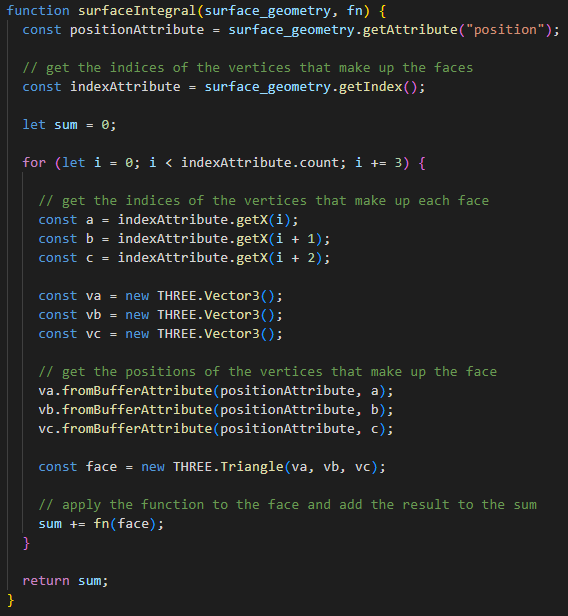
\includegraphics[width=0.8\textwidth]{images/surface_int.png}
    \caption{Surface Integral of a Scalar Field\cite{El-Deeb_PEU-218_Stokes_Threejs}}
\end{figure}

As it can be seen, the surface integral of a scalar field is approximated by summing up the values of the scalar field over many small triangles on the surface.

\begin{figure}[H]
    \centering
    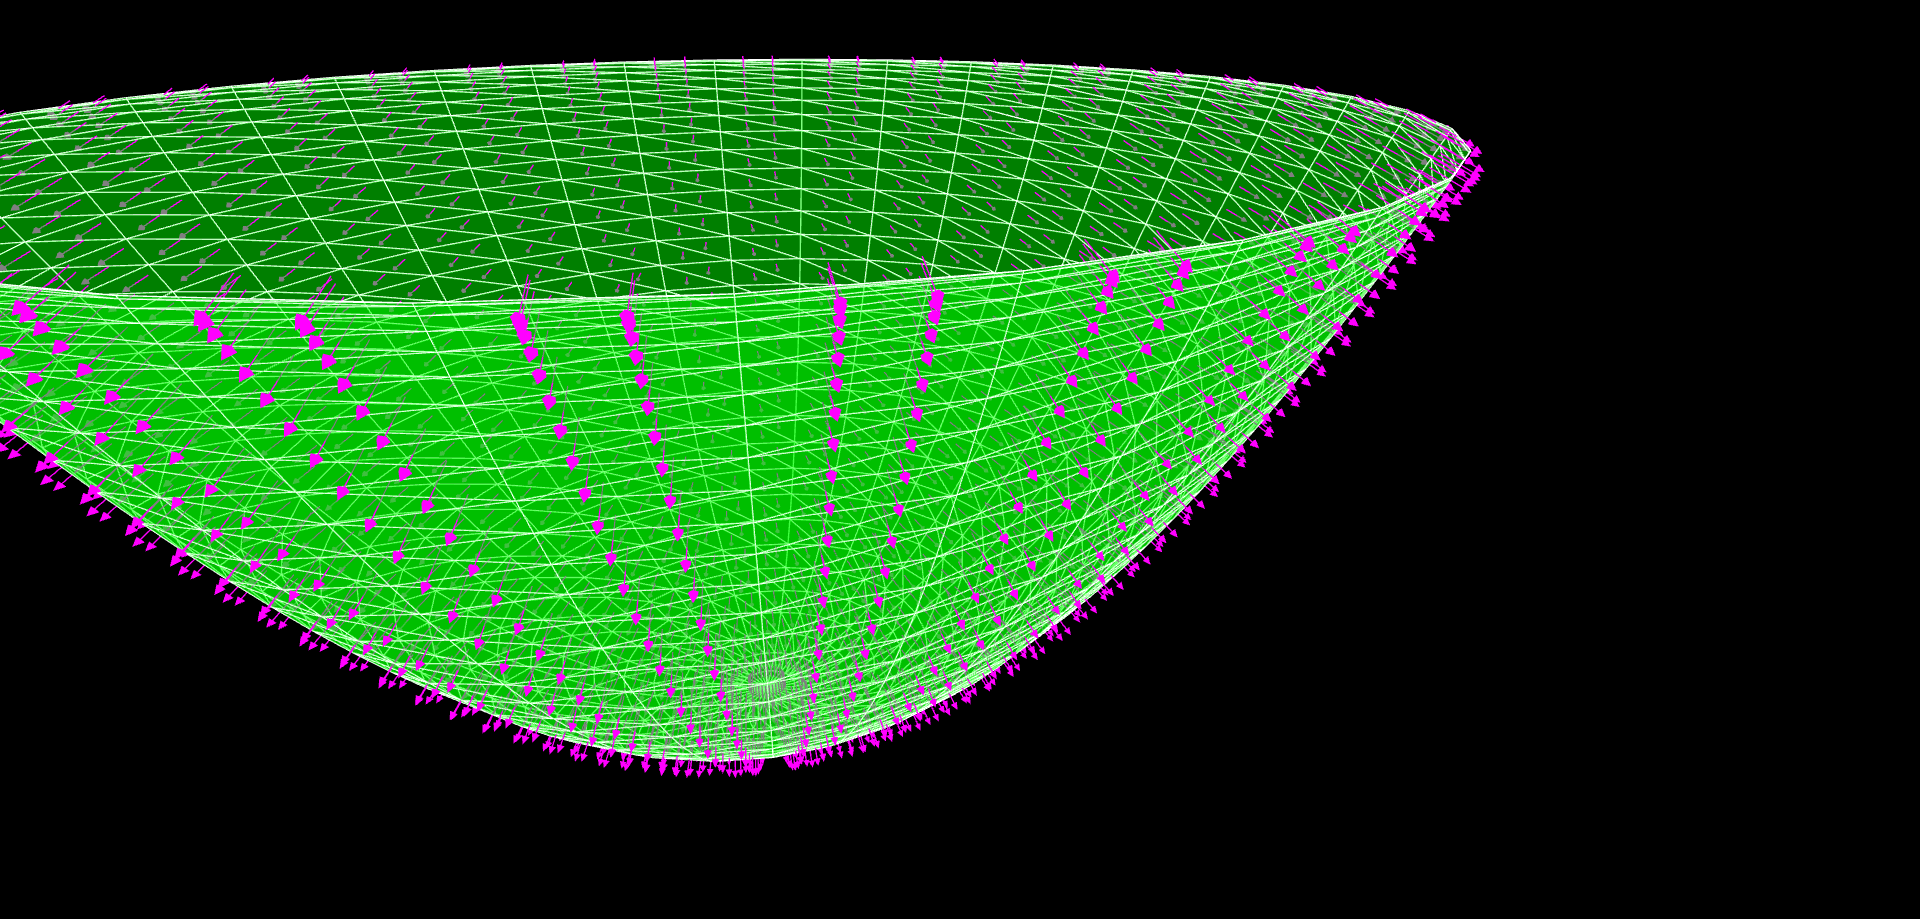
\includegraphics[width=0.8\textwidth]{images/surface.png}
    \caption{Triangle mesh and surface normals of the surface of a paraboloid\cite{El-Deeb_PEU-218_Stokes_Threejs}}
\end{figure}

This integration method is used to compute the surface integral side of Stokes' curl theorem.

\newpage
\section{Scaler Field}
\subsection{Definition}

A scalar field is a function that assigns a scalar value to every point in space. The value may be constant or vary over time and space. Mathematically, a scalar field can be represented as:

\[
    f: \mathbb{R}^3 \rightarrow \mathbb{R}
\]

This is trivial to implement in code as it is just a function that takes a 3D point as input and returns a scalar value.
the only issue is to be able to handle singular points where the function is not defined.

We may want to visualize the scalar field and numerous ways to do so, one way is to use a color map to represent the scalar value at each point. We can use the \href{https://en.wikipedia.org/wiki/Heat_map}{heat map} color map where the color represents the value of the scalar field at each point.
In that case we would need to pre-compute the scalar field to find the minimum and maximum values to normalize the color map. if the field is 2D we plot it on a 3D surface where the height of the surface represents the value of the scalar field at each point.

\subsection{Implementation}

The implementation of a scalar field is straightforward, we can implement the scalar field as a class that contains an arbitrary function and a method that takes a 3D point as input and returns a scalar value.
And class methods to represent other operations on the scalar field such as the partial derivatives and the gradient.

\subsection{Partial Derivatives of a Scalar Field}

\subsubsection{Definition}

The partial derivatives of a scalar field are the derivatives of the scalar field with respect to each of the independent variables. The partial derivatives are defined as:

\[
    \frac{\partial f}{\partial x}, \quad \frac{\partial f}{\partial y}, \quad \frac{\partial f}{\partial z}
\]

We could implement the partial derivatives as functions that take a 3D point as input and return a scalar value.
Where the partial derivatives can be approximated using finite differences.

\[
    \frac{\partial f}{\partial x} \approx \frac{f(x + h, y, z) - f(x - h, y, z)}{2h}
\]

\[
    \frac{\partial f}{\partial y} \approx \frac{f(x, y + h, z) - f(x, y - h, z)}{2h}
\]

\[
    \frac{\partial f}{\partial z} \approx \frac{f(x, y, z + h) - f(x, y, z - h)}{2h}
\]

where \(h\) is the step size. We need to be careful with the step size as it affects the accuracy of the approximation. We want to choose a small step size to get a more accurate approximation but not too small to avoid numerical errors.

\subsubsection{Implementation}

In this program, we can implement the partial derivatives using the finite difference method.

\begin{figure}[H]
    \centering
    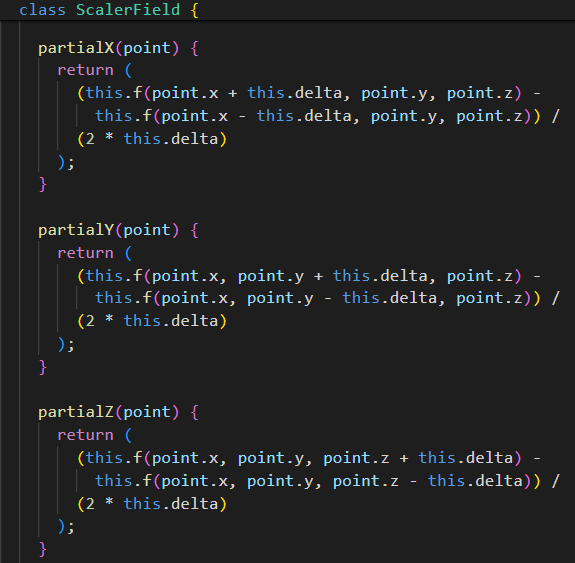
\includegraphics[width=0.8\textwidth]{images/partial.png}
    \caption{Partial Derivatives of a Scalar Field\cite{El-Deeb_PEU-218_Stokes_Threejs}}
\end{figure}

Note: We evaluate the partial derivatives at the center of the cells to get a more accurate approximation.

\subsection{Gradient of a Scalar Field}

\subsubsection{Definition}

The gradient of a scalar field is a vector field that points in the direction of the greatest rate of increase of the scalar field at each point. The gradient is defined as:

\[
    \nabla f = \left\langle \frac{\partial f}{\partial x}, \frac{\partial f}{\partial y}, \frac{\partial f}{\partial z}\right\rangle
\]

We could implement the gradient as a function that takes a 3D point as input and returns a 3D vector.
Where the partial derivatives can be approximated using finite differences.

\subsubsection{Implementation}

The gradient of a scalar field is the an implementation of the partial derivatives of the scalar field.

\begin{figure}[H]
    \centering
    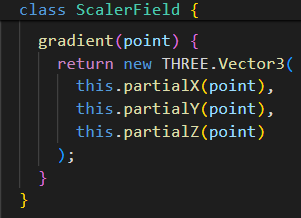
\includegraphics[width=0.8\textwidth]{images/grad.png}
    \caption{Gradient of a Scalar Field\cite{El-Deeb_PEU-218_Stokes_Threejs}}
\end{figure}

\newpage
\section{Vector Field}
\subsection{Definition}

A vector field is a function that assigns a vector to every point in space. The vector may be constant or vary over time and space. Mathematically, a vector field can be represented as:

\[
    \mathbf{F}: \mathbb{R}^3 \rightarrow \mathbb{R}^3
\]

This is also trivial to implement in code as it is just a function that takes a 3D point as input and returns a 3D vector.

Note that vector fields can for all intents and purposes be treated as n scalar fields where n is the dimension of the vector field. The will come in when we discuss the divergence and curl of a vector field.

To visualize a vector field, we can use arrows to represent the vectors at each point. The length of the arrow represents the magnitude of the vector and the direction of the arrow represents the direction of the vector. We can also use color to represent the magnitude of the vector and in that case we could normalize the arrows to have the same length.
There are two common way to visualize a vector field, the first is to plot the vectors starting from the sampled points and the second is to plot the vectors at the center of the cells.
The difference only amounts to a shift in the position of the vectors by half its length parallel to its direction.

\subsection{Implementation}

\subsection{Divergence of a Vector Field}

\subsubsection{Definition}

The divergence of a vector field is a scalar field that represents the rate at which the vector field is expanding at each point. The divergence is defined as:

\[
    \nabla \cdot \mathbf{F} = \frac{\partial F_x}{\partial x} + \frac{\partial F_y}{\partial y} + \frac{\partial F_z}{\partial z}
\]

Since in divergence we are dealing with each component of the vector field separately, we could treat each component as a scalar field and we just compute the partial derivate of that component with respect to the corresponding axis.
Then we sum up the partial derivatives of each component to get the divergence.

\subsubsection{Implementation}

\subsection{Curl of a Vector Field}

\subsubsection{Definition}

The curl of a vector field is a vector field that represents the rotation of the vector field at each point. The curl is defined as:

\[
    \nabla \times \mathbf{F} = \left\langle \frac{\partial F_z}{\partial y} - \frac{\partial F_y}{\partial z}, \frac{\partial F_x}{\partial z} - \frac{\partial F_z}{\partial x}, \frac{\partial F_y}{\partial x} - \frac{\partial F_x}{\partial y}\right\rangle
\]

We can use the same approach as the divergence to compute the curl. We treat each component of the vector field as a scalar field and compute the partial derivatives of each component with respect to the specified axes.
Then we arrange the partial derivatives in the correct order to get the curl.

\subsubsection{Implementation}

\newpage
\section{Result}



\subsection{Verification of Stokes' Curl Theorem}

There are many ways to verify the correctness of the implementation, one way is to compare the numerical results with the analytical solutions.

\subsubsection{Example 1}

A triangle with vertices \((0, 0, 3), (0, 2, 0)\) and \((4, 0, 0)\) in the \(x y\)-plane. The vector field is \(\vec{F}=\left(3 y x^2+z^3\right) \hat{\imath}+y^2 \hat{\jmath}+4 y x^2 \hat{k}\).
And the rotation is counter clockwise if you are above the triangle and looking towards the \(x y\)-plane.

The analytical solution is:

\[
    \iint_S \vec{\nabla} \times \overrightarrow{\boldsymbol{u}} \cdot \widehat{\boldsymbol{n}} d S=\oint_C \overrightarrow{\boldsymbol{u}} \cdot d \vec{r}
\]

\[
    \vec{\nabla} \times \vec{F} =
    \begin{vmatrix}
        \hat{\imath}                & \hat{\jmath}                & \hat{k}                     \\
        \frac{\partial}{\partial x} & \frac{\partial}{\partial y} & \frac{\partial}{\partial z} \\
        3 y x^2 + z^3               & y^2                         & 4 y x^2
    \end{vmatrix}
    = 4 x^2 \hat{\imath} + \left(3 z^2 - 8 x y\right)  \hat{\jmath} - 3 x^2 \hat{k}
\]

The normal of the triangle is same as the normal of the plane that passes through the three vertices of the triangle.

The equation of the plane is

\[
    \frac{x}{4} + \frac{y}{2} + \frac{z}{3} = 1
\]

The normal of the plane and the triangle is

\[
    \vec{n} = \left( \frac{1}{4}, \frac{1}{2}, \frac{1}{3} \right)
\]

\[
    \hat{n} = \frac{\vec{n}}{\left| \vec{n} \right|}
    = \frac{\frac{1}{4} \hat{\imath} + \frac{1}{2} \hat{\jmath} + \frac{1}{3} \hat{k}}{\sqrt{\frac{1}{16} + \frac{1}{4} + \frac{1}{9}}}
    = \frac{3 \hat{\imath} + 6 \hat{\jmath} + 4 \hat{k}}{\sqrt{61}}
\]

\[
    \vec{\nabla} \times \vec{F} \cdot \hat{n}
    = \left(
    4 x^2 \hat{\imath}
    + \left(3 z^2 - 8 x y\right) \hat{\jmath}
    - 3 x^2 \hat{k}
    \right) \cdot
    \frac{3 \hat{\imath} + 6 \hat{\jmath} + 4 \hat{k}}{\sqrt{61}}
\]

\[
    = \frac{12 x^2 + 18 z^2 - 48 x y - 12 x^2}{\sqrt{61}}
    = \frac{18 z^2 - 48 x y}{\sqrt{61}}
\]

\[
    \iint_S \vec{\nabla} \times \vec{F} \cdot \hat{n} d S
    = \frac{6}{\sqrt{61}} \iint_S \left(3 z^2 - 8 x y\right)  d S
\]

\[
    \iint_S f(x, y, z) d S= \iint_D f(x, y, g(x, y))|\vec{\nabla} \emptyset| d x d y
\]

\[
    g(x, y) = 3 - \frac{3}{4} x - \frac{3}{2} y
\]

\[
    \emptyset = z - 3 + \frac{3}{4} x + \frac{3}{2} y
\]

\[
    \vec{\nabla} \emptyset = \left( \frac{3}{4}, \frac{3}{2}, 1 \right)
\]

\[
    |\vec{\nabla} \emptyset| = \sqrt{{\left( \frac{3}{4} \right)}^2 + {\left( \frac{3}{2} \right)}^2 + 1^2}
    = \sqrt{\frac{9}{16} + \frac{9}{4} + 1}
    = \sqrt{\frac{9 + 36 + 16}{16}}
\]

\[
    = \sqrt{\frac{61}{16}}
    = \frac{\sqrt{61}}{4}
\]

\[
    \iint_S \vec{\nabla} \times \vec{F} \cdot \hat{n} d S
    = \frac{3}{2} \int_0^2 \int_0^{4-2y} \left(\frac{27}{16} {\left(x + 2y - 4\right)}^2 - 8 x y\right)  dx dy
\]


\[
    = \frac{3}{2} \int_0^2 {\left[\frac{27}{48} {\left(x + 2y - 4\right)}^3 - 4 x^2 y\right]}_0^{4-2y} dy
\]

\[
    = - \frac{3}{2} \int_0^2 {\left(16 {\left(y-2\right)}^2 y + \frac{27}{6} {\left(y - 2\right)}^3\right) } dy
\]

\[
    = - \frac{3}{2} \int_0^2 {\left(16 \left(y^3-4y^2+4y\right) + \frac{27}{6} {\left(y - 2\right)}^3\right) } dy
\]

\[
    = - \frac{3}{2} {\left[16 \left(\frac{y^4}{4}-\frac{4}{3}y^3+2y^2\right) + \frac{27}{24} {\left(y - 2\right)}^4\right] }_0^2
\]

\[
    = - \frac{3}{2} \left(16 \left(\frac{16}{4}-\frac{32}{3}+8\right) - \frac{27*16}{24}\right)
\]

\[
    = - 5
\]

The numerical solution is:

-5.0018 for the path integral and -5.0014 for the surface integral on a step size of 128.

\subsubsection{Example 2}

Lets take S to be the upper half surface of a sphere of radius 1 centered at the origin. The vector field is \(\vec{F} = \left(2x-y, -yz^2, -y^2z\right)\).

The analytical solution is:

\[
    \vec{r}=\langle\cos t, \sin t, 0\rangle, 0 \leq t \leq 2 \pi
\]

\[
    d \vec{r}=\langle-\sin t, \cos t, 0\rangle d t
\]

\[
    \vec{A}(t)=\langle 2 \cos t-\sin t, 0,0\rangle
\]

\[
    \vec{A} \cdot d \vec{r}=\left(-2 \cos t \sin t+\sin ^2 t\right) d t
\]

\[
    \oint_C \vec{A} \cdot d \vec{r}=\int_0^{2 \pi}\left(-2 \cos t \sin t+\sin ^2 t\right) d t=\left[-2 \frac{\sin ^2 t}{2}\right]_0^{2 \pi}+\frac{1}{2} \int_0^{2 \pi}(1-\cos 2 t) d t
\]

\[
    \oint_C \vec{A} \cdot d \vec{r}=0+\frac{1}{2}\left[t-\frac{\sin 2 t}{2}\right]_0^{2 \pi}=\pi
\]

The numerical solution is:

3.1403 for the path integral and 3.1403 for the surface integral on a step size of 128.

\subsection{Discussion}

This system is a simple framework that can be extended to include more features and optimizations. The system can be extended to include more vector and scalar field operations and more visualization options. The system can also be optimized to handle larger data sets and more complex vector fields.
A useful optimization would be to use a more accurate method to compute the partial derivatives such as symbolic differentiation. Another optimization would be to use a more efficient method to compute the divergence and curl of the vector field such as the finite element method\cite{FEM} or the finite volume method\cite{Finite_Volume_Methods}.
A rigorous numerical analysis of the system would be useful to determine the accuracy and stability of the system. The system could also be extended to include more vector calculus theorems and operations such as the gradient theorem, the divergence theorem, and the Laplacian operator.
A better tilling algorithm could be used to sample the surface at a more uniform intervals.


\newpage
\section{Conclusion}

In this project, we have built a simple vector calculus framework to verify and visualize Stokes' curl theorem using basic numerical methods and the web graphics library three.js. We have implemented the integration of a scalar field over a path and a surface, the partial derivatives of a scalar field, the gradient of a scalar field, the divergence of a vector field, and the curl of a vector field. We have also visualized the vector field using arrows. We have verified the correctness of the implementation by comparing the results with the analytical solution. The system can be extended to include more features and optimizations and can be used to study more vector calculus theorems and operations.

\newpage
\section{References}
\bibliographystyle{plain}
\bibliography{references}

\end{document}